% !TEX root = main.tex

Buildings are at the heart of society and currently account for 32\% of global final energy consumption and 19\% of energy related greenhouse gas emissions \cite{IPCC}. Nevertheless the building sector has a 50-90\% emission reduction potential using existing technologies, and widespread implementation could see energy use in buildings stabilise or even fall by 2050 \cite{IPCC}. Within this strategy, building integrated photovoltaics (BIPV) has the potential of providing a substantial segment of a building's energy needs \cite{defaix2012technical}. Even the photovoltaic (PV) industry has identified BIPV as one of the four key factors for the future success of PV \cite{raugei2009life}. \\

Recent developments regarding efficiency and costs of thin film BIPV technologies, in particular, CIGS, have brought new design possibilities \cite{NREL, kushiya2014cis, kaelin2004low, jelle2012building}. Their lightweight nature and customisable shapes allow for easier and more aesthetically pleasing integration into the building envelope. In addition, less power is required to actuate them, thus facilitating the development of dynamic envelope elements due to their reduced weight \cite{rossi2012adaptive}. \\





Dynamic buildings envelopes have gained interest in recent years because they can save energy by controlling direct and indirect radiation into the building, while still responding to the desires of the user \cite{loonen2013climate}. This mediation of solar insolation can offer a reduction in heating / cooling loads and an improvement of daylight distribution as seen in Figure \ref{fig:ASFschematic4} \cite{rossi2012adaptive}. Interestingly the structure and mechanics required for dynamic envelopes couples seamlessly with the structure and mechanics required for facade integrated PV solar tracking. The use of light weight PV as an adaptive envelope material enables it to also benefit from on-site energy production. Furthermore, it provides a new way of aesthetically integrating PV panels onto buildings. The balance of electricity production and adaptive shading can in some cases offset the entire energy demand of an office space behind the envelope \cite{jayathissa2015abs}. We have proposed one possible combination of these technologies as an Adaptive Solar Facade (ASF) \cite{nagy2016adaptive}. An example of an ASF can be seen in Figure \ref{fig:HoNR4}.




\begin{figure}
\begin{center}
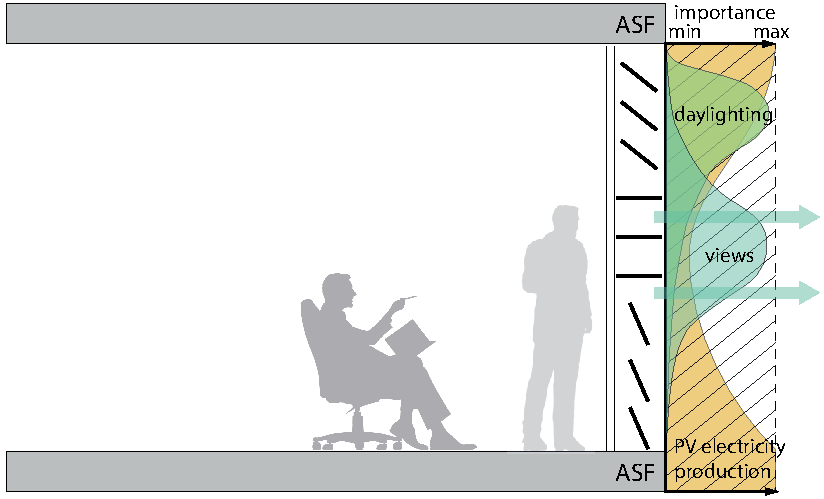
\includegraphics[width=8cm, trim= 0cm 0cm 0cm 0cm,clip]{facadeFunctions.pdf}
\caption{The facade acting as a mediator between the interior and exterior environment, while fullfilling various functions \cite{nagy2016adaptive}}
\label{fig:ASFschematic4}
\end{center}
\end{figure}

\begin{figure}
\begin{center}
\includegraphics[width=8cm, trim= 0cm 0cm 0cm 0cm,clip]{honr.jpg}
\caption{An example of an ASF constructed at the House of Natural Resources \cite{nagy2016adaptive}}
\label{fig:HoNR4}
\end{center}
\end{figure}

The design of an ASF comes at an added cost. The additional electronics, actuators, and supporting structure adds further embodied CO$_2$ to the product. It is therefore important to conduct a life cycle impact assessment (LCA) to analyse whether the life cycle environmental impacts are favorable, compared to a more classic system. It is also important to see how variations in design can alter the green house gas (GHG) reduction potential of the technology. Aspects such as the chosen actuator, control system, and location of operation can have an impact on environmental performance. 

The state of the art literature assesses existing photovoltaic technologies \cite{raugei2007life, de2013energy, fthenakis2011photovoltaics}, and the balance of systems (BOS) which includes all other components of a photovoltaic system \cite{mason2006energy}. This has not however, been expanded to dynamic BIPV systems, and in particular, systems that combine the benefits of adaptive shading and electricity production.\\


In this paper, we investigate the environmental performance of an ASF and compare it to existing static photovoltaic systems. We also investigate 1) a system expansion including the heating ventilation and air conditioning (HVAC) savings through adaptive shading 2) design variations of the ASF, 3) the operational emissions of a building, with and without an ASF, and 4) the sensitivity of the LCA to its location and design.



The remainder of the paper is organized as follows. The following section introduces the ASF and the used LCA methodology. In Section \ref{ch:results4}, we present the results of the LCA analysis. Section \ref{ch:discussion4} discusses the results and provides design guidelines. Section \ref{ch:conclusion4} concludes the paper.

